\chapter{Hardware counterfeiting}
One of the main issues related to hardware security is \textbf{trust}, after all, how can we be sure 
that the hardware we are using is the one we think it is?\\
We will see that there are many different kinds of counterfeiting, which is an actual threat: from
2007 to 2012, one counterfeit part was found every 15 seconds, with an estimated cost of 169 billion
dollars for the whole supply chain.
\begin{section}{Counterfeit types}
  There are many different kinds of counterfeiting, which can be classified as in figure 
  \ref{fig:counterfeit-types}.
  \begin{figure}[H]
    \centering
    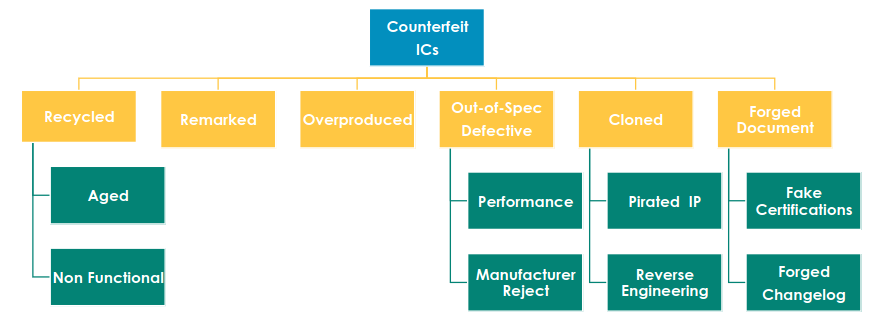
\includegraphics[width=0.8\textwidth]{img/hardware/counterfeit types.png}
    \caption{Counterfeit types}
    \label{fig:counterfeit-types}
  \end{figure}

  \begin{subsection}{Recycled parts}
    Recycled parts are parts that have been used, removed from the original system, and then sold as
    new.\\
    An electronic component recovered from a scrap board can be sold as new by modifying it to be 
    misrepresented as a new one. This is a common practice in the industry, and it's a real threat.
    There are two main concerns about recycled parts:
    \begin{itemize}
      \item \textbf{Safety}: the component has already aged, which results in a shorter lifespan and
        to possible lower performance. Furthermore, it could have been damaged during the removal
        process(removal under very high temperatures, aggressive physical removal from boards,
        washing, sanding, repackaging, etc.)
      \item \textbf{Security}: an old hardware sold as new could have unpatched vulnerabilities, which
        could be exploited by an attacker.
    \end{itemize}
    The failure rate of a ic component would be represented by the \textbf{bathtub curve}, which
    is shown in figure \ref{fig:bathtub-curve}.
    \begin{figure}[H]
      \centering
      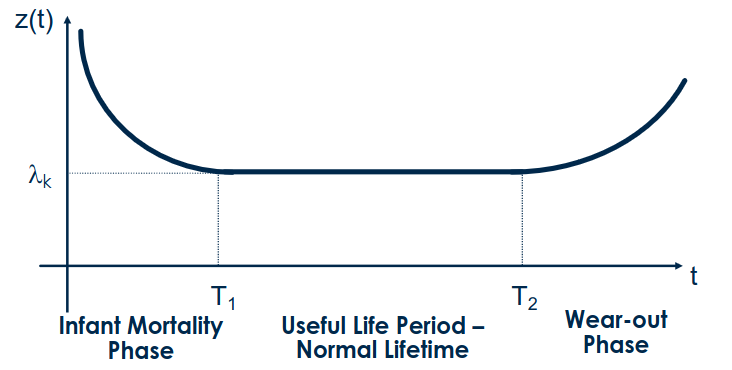
\includegraphics[width=0.5\textwidth]{img/hardware/bathub curve.png}
      \caption{Bathtub curve}
      \label{fig:bathtub-curve}
    \end{figure}
    As you could have already imagined, the failure rate at the end of the useful life of the 
    component is higher, and a recycled part would most likely be in this phase.
  \end{subsection}
  \begin{subsection}{Remarked parts}
    Remarked parts are parts from which the original marking( the logo, the part number, etc.) has
    been chemically or mechanically removed.\\
    This is done for two main reasons:
    \begin{itemize}
      \item drive up the component's price on the open market
      \item make dissimilar lot fraudulently appear homogeneous
    \end{itemize}
  \end{subsection}
  \begin{subsection}{Overproduced parts}
    Overproduced parts are parts that are produced in excess by the original manufacturer and then
    sold on the open market, outside of the contract with the design house parts.\\
    This practice causes a loss of revenue for the designer and the IP owner, but also a reliability 
    issue, as the parts are not tested and validated as the original ones.
  \end{subsection}
  \begin{subsection}{Cloned Components}
    Cloned components are parts that are produced by a third party produced it without the original
    manufacturer's consent to eliminate the development costs.\\
    The cloning portion could be done in different ways:
    \begin{itemize}
      \item \textbf{Reverse engineering}: the component is analyzed, and the design is copied
      \item \textbf{IP theft}: the design is stolen from the original manufacturer
      \item \textbf{Insider leak}: the knowledge if transferred in an unauthorized way by a person
        with access to the design
    \end{itemize}
    Cloned electronics these days are potentially more nefarious: counterfeiters make their
    components, boards, and systems from scratch and package them into superficially similar
    products.\\
    The clones may be less reliable than the genuine product, having never undergone rigorous
    testing. ,but they may also host unwanted or malicious software, firmware, or hardware — and the
    buyer may not know the difference or even know what to look for.
  \end{subsection}
  \begin{subsection}{Tampered components}
    Tampered components are parts that have been modified to cause damage or make unauthorized 
    changes to the system.\\
    Most commonly, they are used to insert a backdoor in the system.
  \end{subsection}
\end{section}

\begin{section}{Counterfeit Detection}
  There are different ways to detect counterfeit components, which can be classified as in figure 
  \ref{fig:counterfeit-detection}.
  \begin{figure}[H]
    \centering
    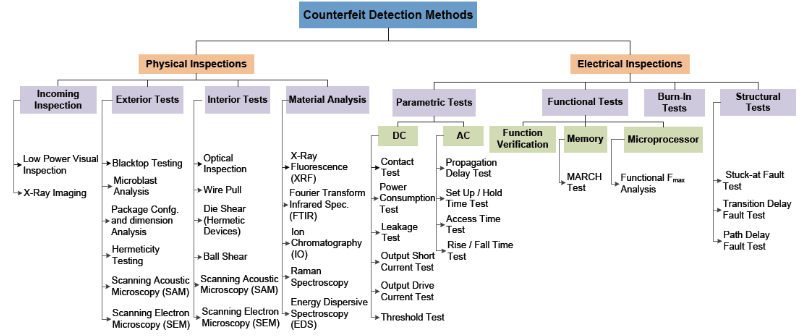
\includegraphics[width=0.8\textwidth]{img/hardware/counterfeit detection.png}
    \caption{Counterfeit detection}
    \label{fig:counterfeit-detection}
  \end{figure}
  We will go over only some of them, based on the defect that they are looking for.\\
  Recycled parts usually presents \textbf{texture variations}(see figure
  \ref{fig:texture-variations}) due to the sanding, remarking, or resurfacing, but those are
  believed to be some of the most frequent but yet challenging to detect phenomena in counterfeit
  ICs. The \textbf{oxidation effect}(see figure \ref{fig:oxidation-effect}) is another common 
  defect, which is caused by the exposure to the environment without proper protection for a long
  time.\\
  \textbf{Contamination}(see figure \ref{fig:contamination-effect}) could be another indicator of a recycled
  part, as well as \textbf{ghost markings}(see figure \ref{fig:ghost-markings}), which appear when the
  counterfeiters do no remove entirely the original markings before printing the new ones.\\
  An unclean device could be a sign of a recycled part too, or maybe some imprints only visible
  under a microscope, like the year of production, the manufacturer, or the country of origin.

  \begin{figure}[H]
    \centering
    \begin{subfigure}{0.4\textwidth}
      \centering
      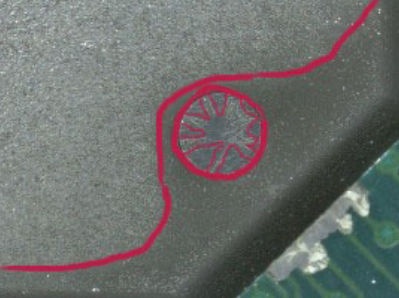
\includegraphics[width=\textwidth]{img/hardware/texture variation.png}
      \caption{The damage cause by the removal process}
      \label{fig:texture-variations}
    \end{subfigure}
    \begin{subfigure}{0.4\textwidth}
      \centering
      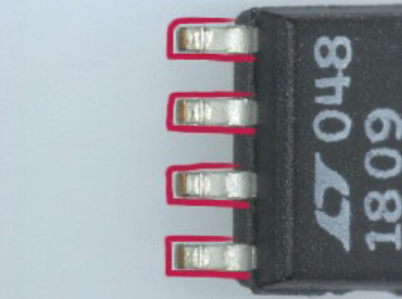
\includegraphics[width=\textwidth]{img/hardware/oxidation effect.png}
      \caption{The oxidation effect}
      \label{fig:oxidation-effect}
    \end{subfigure}
    \begin{subfigure}{0.4\textwidth}
      \centering
      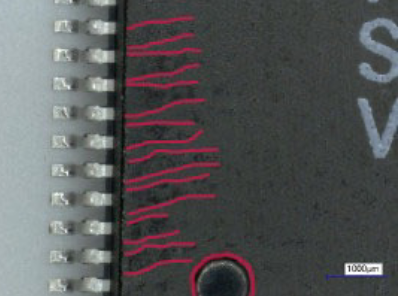
\includegraphics[width=\textwidth]{img/hardware/contamination effect.png}
      \caption{The effect of contamination}
      \label{fig:contamination-effect}
    \end{subfigure}
    \begin{subfigure}{0.4\textwidth}
      \centering
      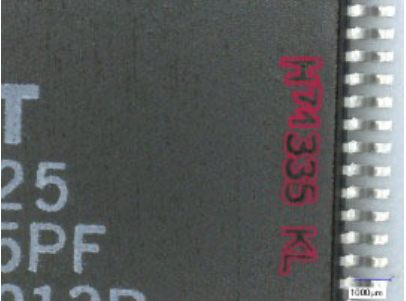
\includegraphics[width=\textwidth]{img/hardware/ghost markings.png}
      \caption{Ghost markings left by the removal process}
      \label{fig:ghost-markings}
    \end{subfigure}
    \caption{Various effect on recycled parts}
  \end{figure}
\end{section}

\begin{section}{Counterfeiting Prevention}
  The are quite a few methods to prevent counterfeiting.
  \begin{subsection}{Aging Detection}
    Aging detection are made up of sensors in the chip, used to capture the usage of the component.
    They rely on the aging effects of MOSFETs to change a ring oscillator frequency in comparison
    with the golden one embedded in the chip.\\
    They can also be made up of antifuse-based technology to record the usage time of the component.
  \end{subsection}

  \begin{subsection}{Hardware Metering}
    Hardware metering refers a set of security protocols that enable the design house to achieve the
    post- fabrication control of the produced ICs to \textbf{prevent overproduction}.
    Some example of this are:
    \begin{itemize}
      \item Post-manifacturing activation of the ICs
      \item Adding a Finite-State Machine (FSM) which is initially locked and can be unlocked only
        with the correct sequence of primary inputs(which is basically watermarking)
      \item Logic encryption
    \end{itemize}
  \end{subsection}
  \begin{subsection}{PUF}
    PUFs are a good way to prevent counterfeiting, as they are unique to each device and can be used
    to identify it without the need to program the ID value or store it.\\
    Implementing a puf assures that non reverse engineering can be done, and the device cannot be
    cloned.
  \end{subsection}
\end{section}
